\Chapter{Neurális hálók}

A neurális hálózattokat gyakran hasonlítjuk az emberi agy működéséhez. Ha körültekintően szemügyre vesszük agyunk működését, akkor azt tapasztaljuk, hogy neuronokból és közöttük felépülő kapcsolatokból áll össze. A külvilágból érkezett ingereket értelmezhetjük úgy, mint egy bemenetet, amit az agyunkban lévő neuronok feldolgoznak.\\

\begin{center}
	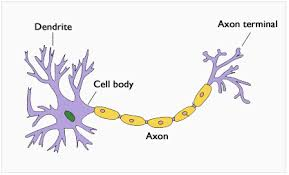
\includegraphics[scale=1.0]{neuron}
\end{center}

A kutatók az agy felépítését vizsgálva egy olyan matematikai modellt dolgoztak ki, amely   reprezentálni próbálja az agyban található neuronokat és a közöttük lévő kapcsolatokat. Ezt a modellt nevezzük neurális hálónak vagy neurális hálózatnak.\\

A neurális hálózatot alkotó neuronok úgynevezett rétegekbe rendeződnek. Háromféle réteget különbözetünk meg, a \textbf{\textit{bemeneti}}, a \textbf{\textit{kimeneti}} és a \textbf{\textit{rejtett réteget}}. Bemeneti és kimeneti rétegből minden hálózatban egy darab van, rejtett rétegből azonban tetszőleges számú lehet.\\

A hálózatban a rétegeket élek kötik össze egymással, amelyekhez egyenként egy-egy \textbf{\textit{súly}} tartozik. A neuronok a bemeneti éleiken kapott értékek és a súlyok segítségével bizonyos műveleteket végeznek el, majd az eredmény a kimeneti éleiken keresztül továbbítják a következő réteg neuronjai felé.\\

A tanítási folyamat elvégzésekor a hálózatba olyan bemenetet juttatunk, amelyhez tartozó kimenet ismert. A bemenetet végig futtatjuk a hálózat rétegein, majd a kimeneti réteg által szolgáltatott eredményt összehasonlítjuk a kimenet várt értékével. A két érték közötti eltérést a hálózat \textit{\textbf{hibájának}} nevezzük. A tanítás folyamán a hálózat súlyait úgy változtatjuk, hogy ez a hiba lehetőleg minél kisebb legyen. A hálózat betanítása után már olyan bemeneteket is megadhatunk, amelyeknek már nem ismerjük a kimenetét, és a hálózat ezekre is képes hibahatáron belüli kimenetet produkálni.

\begin{figure}
	\centering
	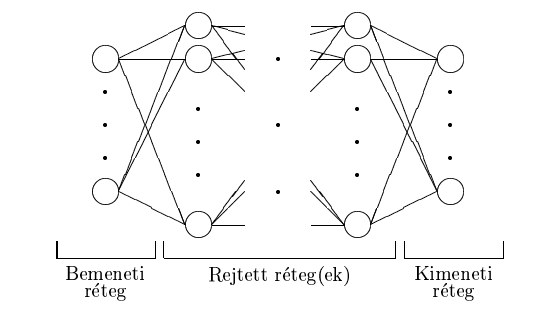
\includegraphics[scale=0.75]{ANNLayers}
	\caption{Egy általános felépítésű neurális hálózat}
\end{figure}

\begin{flushleft}
{\Large Perceptron}\\
\end{flushleft}

Az egyszerűség kedvéért vizsgáljunk meg egy olyan neurális hálózatot, amelynek egyetlen neuronnal rendelkezik. Ezt szokás \textbf{\textit{Perceptron}}-nak is nevezni.

\begin{flushleft}
\textit{\textbf{{\large Részei:}}}
\end{flushleft}

\textbf{\textit{Bemenet}}: Az kiértékelendő adat (ember számára ingerek), amit általában egy vektor (\(x\)) reprezentál.\\

\textit{\textbf{Súlyok}}: Két neuron közötti kapcsolat. Egy valós szám (eleinte véletlenszerűek). A hálózat súlyait (W) mátrixba tároljuk el.\\

\textbf{\textit{Összegző csomópont}}: A bemeneteket összeszorozza a megfelelő súlyokkal és ezek összegét képezi. Tulajdonképpen mátrix szorzásról van szó.

\[v(n) = \sum_i^{n}(w_ix_i)\]

\textit{\textbf{Aktivációs függvény}}: Egy olyan függvény ($\varphi$), ami leképezi a kapott összeget egy kisebb intervallumba pl. [0,1] vagy [-1,1] között.\\

\textbf{\textit{Kimenet}}: A leképezett értékünk lesz a kimenetünk (\(y\)).\\

\begin{center}
	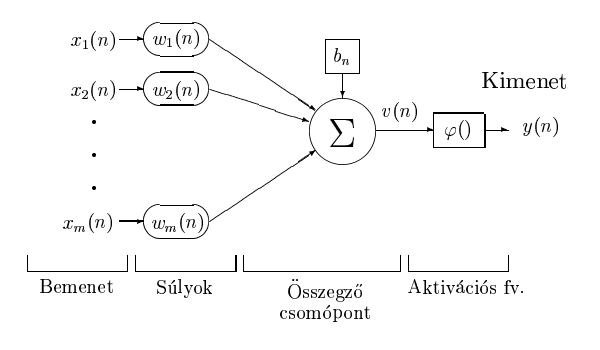
\includegraphics[scale=0.6]{ANNParts}
\end{center}

\marginnote{\textit{Mi lenne ha az összes generált súly 0 értékű?}}[-0.66cm]

A képen láthatunk egy \(b_n\) változot másnéven bias, amit most nem részleteznék. Alapvetően arra való hogy aktiváljon egy neuront. A \(b(n)\)-hez tartozó súly (\(w_b\)) általában -1 vagy 1.\\

Amennyiben az \(x(n)\) bemenethez tartozó ideális kimenetet \(d(n)\)-nel jelöljük, illetve \(y(n)\) jelenti a hálózat által az \(x(n)\) bemenetre adott kimenetét, a neurális hálózat négyzetes hibáját a következőképpen értelmezzük:

\[ \varepsilon = (d(n) - y(n))^2\]

Ezt a hibát akarjuk a tanítási eljárás során minimálisra csökkenteni. Természetesen az lenne az ideális, ha a hibát egészen nullára tudnánk redukálni, de ez általában nem sikerül, ezért meg kell elégednünk egy kellően kicsiny hibaküszöbbel.\\

Aktivációs függvényként tetszőleges balról illetve jobbról folytonos eloszlásfüggvény megfelel, azaz olyan függvényt kell választanunk, amely

\begin{itemize}
\item monoton növekvő
\item balról/jobbról folytonos,
\item határértéke + $\infty$ -ben 1, - $\infty$ -ben 0.
\end{itemize}

Aktivációs függvénynek általában a szigmoid, azaz S alakú, függvényeket használjuk (pl. logisztikus, tangens hiperbolikus stb.).\\

Az aktivációs függvényeknél egy ún. rámpafüggvényről (RELU), ami az

\[ f(x) = max(0,x) \]

összefüggéssel írható le, ahol x az aktivációs függvény bemenete.\\

\begin{center}
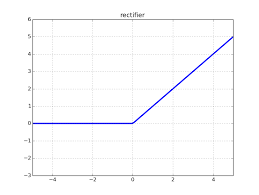
\includegraphics[scale=1.0]{relu}
\end{center}

A legújabb biológiai kutatások és a gyakorlati tapasztalatok is igazolják hogy a RELU-val történő tanítások szignifikánsan jobban teljesítenek. Legnagyobb előnye a regressziós tanítások esetén mutatkozik meg.

\begin{flushleft}
{\Large Backpropagation}\\
\end{flushleft}

Hiba minimalizálása során szükségünk van az aktuális hibára. Az összes kimeneti neuronra kiszámoljuk a négyzetes hibát és ezeket összeadjuk.

\[ E_{total} = \sum \dfrac{1}{2}(target - output)^2\]

\textit{\hl{Az 1/2 szorzót azért használjuk hogy eltávolítsuk a kitevőt, deriváláskor}
}

A backpropagation célja, hogy frissítse az egyes súlyokat a hálózaton úgy, hogy az aktuális kimenet közelebb kerüljön a célkimenethez, ezáltal minimalizálva az egyes kimeneti neuronok és a hálózat egészének hibáját.\\

\begin{center}
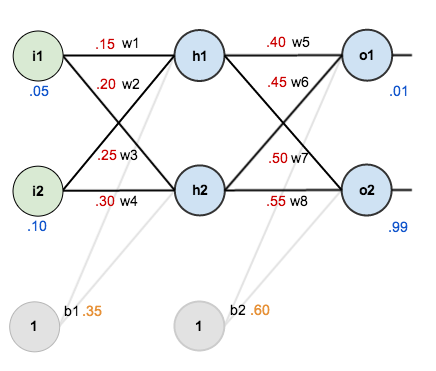
\includegraphics[scale=0.5]{ANN_backprog}
\end{center}

Tekintsük a \(w_5\)-öt. Azt szeretnénk tudni, hogy a \(w_5\) változása milyen hatást gyakorol a teljes hibára, más néven $\frac{\partial E_ {total}}{\partial w_ {5}}$. Úgy is fogalmazhatunk hogy a gradiens a \(w_5\) vonatkoztatásba.\\

A láncszabály alkalmazásával tudjuk kiszámolni:

\[\frac{\partial E_{total}}{\partial w_{5}} = \frac{\partial E_{total}}{\partial out_{o1}} * \frac{\partial out_{o1}}{\partial net_{o1}} * \frac{\partial net_{o1}}{\partial w_{5}}\]

Lássuk az egyenlet elemeit:\\
\begin{flushleft}
\begin{equation}
E_{total} = \frac{1}{2}(target_{o1} - out_{o1})^{2} + \frac{1}{2}(target_{o2} - out_{o2})^{2}
\end{equation}
\begin{equation}
\frac{\partial E_{total}}{\partial out_{o1}} = 2 * \frac{1}{2}(target_{o1} - out_{o1})^{2 - 1} * -1 + 0
\end{equation}
\begin{equation}
\frac{\partial E_{total}}{\partial out_{o1}} = -(target_{o1} - out_{o1}) = -(0.01 - 0.75136507) = 0.74136507
\end{equation}

\end{flushleft}

A logisztikus függvény parciális deriváltja a kimenet szorzata (1 - kimenet):

\[out_{o1} = \frac{1}{1+e^{-net_{o1}}}\]

\[\frac{\partial out_{o1}}{\partial net_{o1}} = out_{o1}(1 - out_{o1}) = 0.75136507(1 - 0.75136507) = 0.186815602\]

Végül, mennyire változik az o1 változó teljes nettó bemenete a \(w_5\) tekintetében?

\[net_{o1} = w_5 * out_{h1} + w_6 * out_{h2} + b_2 * 1\]

\[\frac{\partial net_{o1}}{\partial w_{5}} = 1 * out_{h1} * w_5^{(1 - 1)} + 0 + 0 = out_{h1} = 0.593269992\]

Összesítve:\\

\[\frac{\partial E_{total}}{\partial w_{5}} = \frac{\partial E_{total}}{\partial out_{o1}} * \frac{\partial out_{o1}}{\partial net_{o1}} * \frac{\partial net_{o1}}{\partial w_{5}}\]

\[\frac{\partial E_{total}}{\partial w_{5}} = 0.74136507 * 0.186815602 * 0.593269992 = 0.082167041\]

A hiba csökkentése érdekében kivonjuk ezt az értéket az aktuális súlyból (adott esetben szorozva egy bizonyos tanulási sebességgel, $\eta$, amelyet 0,5-re állítunk):

\[w_5^{+} = w_5 - \eta * \frac{\partial E_{total}}{\partial w_{5}} = 0.4 - 0.5 * 0.082167041 = 0.35891648\]

Meg tudjuk ismételni ezt a folyamatot, hogy megkapjuk az új súlyokat $w_6$, $w_7$ és $w_8$:

\[w_6 ^ {+} = 0,408666186\]

\[w_7 ^ {+} = 0.511301270\]

\[w_8 ^ {+} = 0.561370121\]

Ezután folytatjuk a hátrafelé az új értékeket a $w_1$, $w_2$, $w_3$ és $w_4$ értékek kiszámításával. Hasonlóan láncszabályt alkalmazunk.\\

\begin{center}
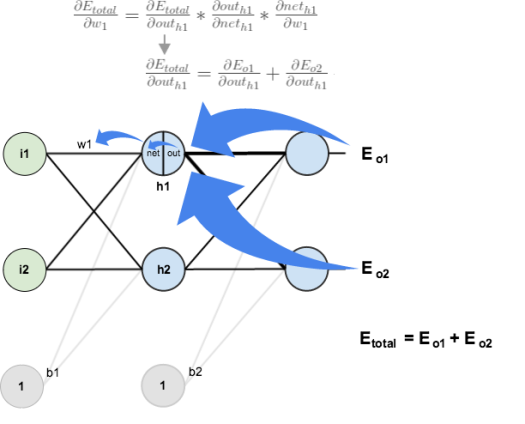
\includegraphics[scale=0.5]{ANN_bp_viz}
\end{center}

Végül frissítjük az összes súlyunkat! Amikor eredetileg a 0.05 és a 0.1 bemeneteket továbbítottuk, a hálózat hibája 0.2983711 volt. A backpropagation első fordulója után a teljes hiba 0,2910279 értékre csökken. Lehet, hogy nem tűnik soknak, de miután megismételtük ezt a folyamatot 10 000-szer, a hiba lecsökken 0,0000351-re.\\

\begin{flushleft}
{\Large Konvolúciós neurális hálózat}\\
\end{flushleft}

A konvolúciós neurális hálózat hagyományos neurális hálózat alapokon nyugszik. Annak egy speciális fajtája, amit képeken található minták feltárására fejlesztettek. Neuronokból épülnek fel és hasonlóképpen rendelkeznek tanítható súlyokkal. A bemeneteiken kapott értékek skaláris szorzatát egy nem lineáris leképezés követheti. Az egész hálózat reprezentálhat egy egyszerű osztályozó eljárást, aminek a bemenetei a nyers képpontok, és a kimenete lehet egy adott kép osztályba tartozás valószínűsége.\\

A hagyományos neurális hálózatok nem skálázzák a teljes képet. Ha példaként vesszük egy 32 pixel széles, 32 pixel magas színes képet és ezt bevezetnénk egy teljesen összekapcsolt rejtett rétegbe, akkor az neurononként 32x32x3 = 3072 súly paramétert jelentene. Ez még kezelhetőnek tűnik, de tisztán látszik, hogy a teljesen összekapcsolt struktúra nem kezeli jól a képeket. Ha példaként megnézünk egy 200x200 méretű színes képet, akkor neurononként 120 000 súly paramétert kapunk. Ha végig gondoljuk, hogy az hány paramétert jelent még egy kis neuronszámú kevés rejtett rétegből álló hálózat esetében, akkor rájöhetünk, hogy nagyobb méretű képen fellelhető minták felismeréséhez a tisztán hagyományos neurális hálózatok alkalmazása nem célravezető, emiatt a kép elő feldolgozására, szűrésére konvolúciós rétegeket vezetnek be.

\begin{flushleft}
\textit{\textbf{Felépítés}}
\end{flushleft}

A konvolúciós neurális hálózatokban szereplő rétegeket funkció alapján alapvetően két csoportra lehet bontani. Az elsőbe sorolhatók a konvolúciós rétegek, amik - mint paraméterezhető szűrők - előfeldolgozást végeznek a képen. Ezáltal a kép mérete lecsökken, a hordozott információtartalom kiemeltté válik, és a hagyományos neurális hálózat (második csoport) számára feldolgozható lesz, az osztályozást el tudja végezni. Egy konvolúciós neurális hálózat tehát konvolúciós és hagyományos rejtett rétegekből épül fel.\\

A konvolúciós rétegek alapjában véve színes képek feldolgozására lettek kifejlesztve, ezért a neuronjaik három dimenzióban (szélesség, magasság, színcsatornák) vannak elrendezve.\\

\begin{center}
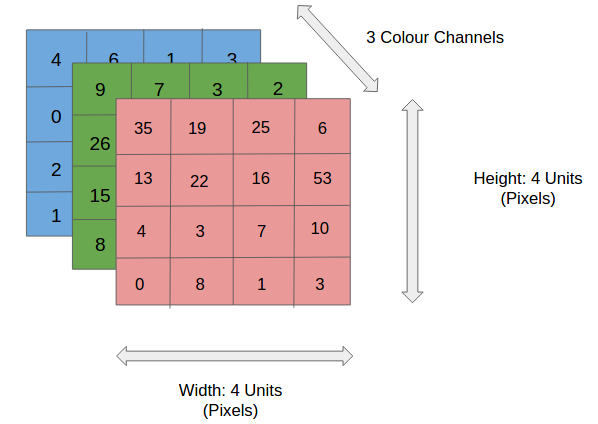
\includegraphics[scale=0.65]{CNN_neuron_channel}
\end{center}

A következő felsorolásban - a tipikus, de nem kizárólagos sorrendre ügyelve - bemutatnám a konvolúciós hálózat rétegtípusait:\\
\begin{itemize}
\item bemeneti réteg: Tartalmazza a kép nyers pixel értékeit, jellemzően R, G, B csatorna szerint rendezve.
\item konvolúciós réteg: Adott képpont csoportokra konvolúció matematikai műveletet alkalmazunk. A konvolúció eredménye egy skalár (a skaláris szorzata a kép egy adott részének és a szűrőnek). Ha minden képpont csoportra elvégezzük a konvolúciót, akkor egy aktivációs térképet kapunk. Általában több szűrő paraméterrel is elvégezzük a konvolúciót és aktivációs térképeket egymásra rakjuk. Az aktivációs térkép, a művelet tulajdonsága miatt, kisebb
méretű lesz.

\begin{center}
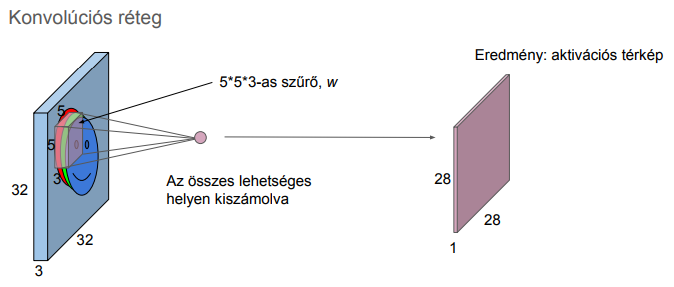
\includegraphics[scale=0.6]{convolution_layer}
\end{center}

\item RELU réteg: A konvolúciós réteg aktivációs függvénye, ami a következő leképezést valósítja meg: \(f(x) = max(x, 0)\). Vagyis, ha a bemenet kisebb, mint nulla, akkor a kimenet nulla lesz, ha nagyobb, mint nulla, akkor a kimenet a bemenet értékét veszi fel.
\item összevonó réteg (pooling layer): Az aktivációs térképekre alkalmazzuk. Csökkenti a reprezentáció méretét, így kezelhetőbbé téve azt. Leskálázza a képet.
\item teljesen összekötött réteg (fully connected, FC): Utolsó rétegekként szokták használni, hagyományos réteg. 
\end{itemize}

A következő ábra egy konvolúciós feldolgozást mutat be, ahol szemléltetve vannak az egyes rétegek utáni állapotok. A képen látható, hogy ez egyes konvolúció utáni állapotok tulajdonság érzékelőként viselkednek.\\

\begin{center}
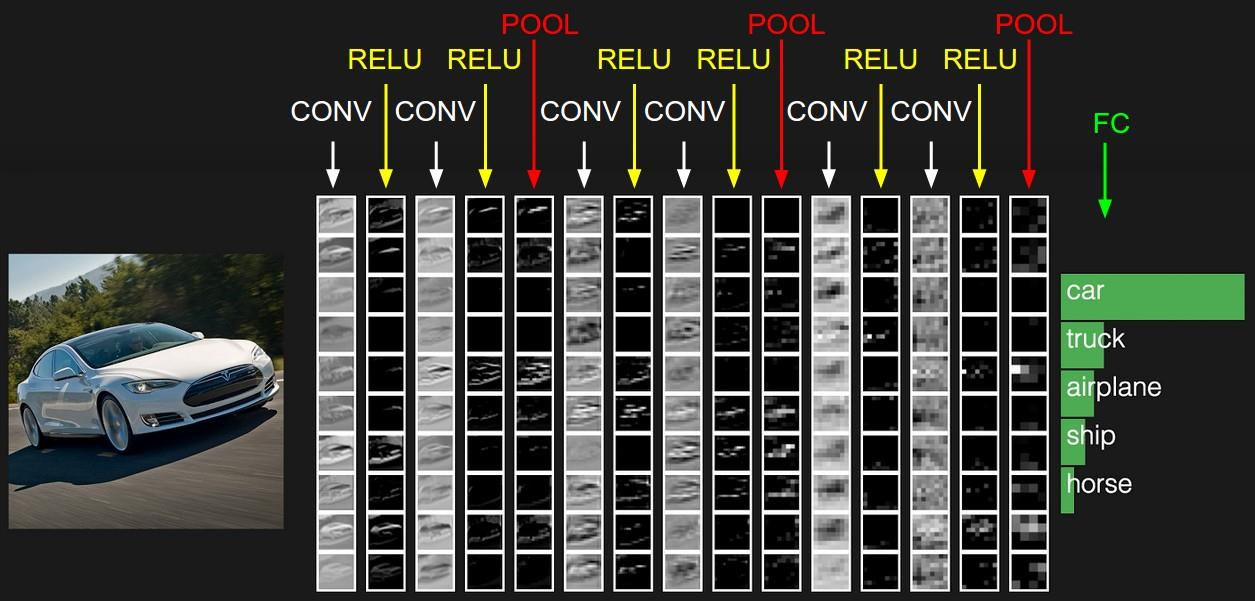
\includegraphics[scale=0.35]{CNN_working}
\end{center}

\begin{flushleft}
{\Large \textit{\textbf{Tanítás}}}
\end{flushleft}

Ez a neurális hálózatok egyik legfontosabb része. Sok kérdés merülhet fel olvasás közben. Hogyan ismerik az első konvolúciós rétegben lévő szűrők az élek és görbék keresését? Hogyan ismeri fel a teljesen összekapcsolt réteg a jellemzőket? Hogyan ismerik a szűrők az egyes rétegekben milyen értékeket kapnak? A számítógép képes beállítani a szűrő értékeit (vagy súlyait) a backpropagation-nek nevezett képzési folyamat révén.\\

A backpropagation négy különböző szakaszra osztható
\begin{itemize}
\item Előre terjesztés (forward pass)
\item Veszteség számítás (loss function)
\item Hiba visszaterjesztés (backward pass)
\item Súly frissítés (weight update)
\end{itemize}

Az előre terjesztés során egy képet (pl. 32x32x3) továbbítunk az egész hálózaton. Az első leképzésnél, mivel minden súly és szűrőérték véletlenszerűen van inicializálva, így a kimenet is valószínűleg véletlenszerű lesz, ezért a hálózat nem add pontos osztályozást. A hálózat jelenlegi súlyaival nem tudja keresni az alacsony szintű jellemzőket. Emiatt tovább lépünk a veszteség számítás részre. Ne felejtsük el, hogy a tanító mintának van egy címkéje. A veszteségfüggvény többféle módon definiálható, de gyakori az MSE (átlagos négyzetes hiba) \(E_{total} = \sum 1/2(target - output)^2\).\\

A veszteség rendkívül magas az első képzésnél. Olyan pontra akarunk jutni, ahol az előre jelzett címke megegyezik a képzési címkével. Ahhoz, hogy odaérjünk, minimálisra csökkentjük a veszteségünket. Azt szeretnénk megtudni, hogy mely bemenetek (súlyok a mi esetünkben) leginkább hozzájárultak a hálózat veszteségéhez (vagy hibájához).

\begin{center}
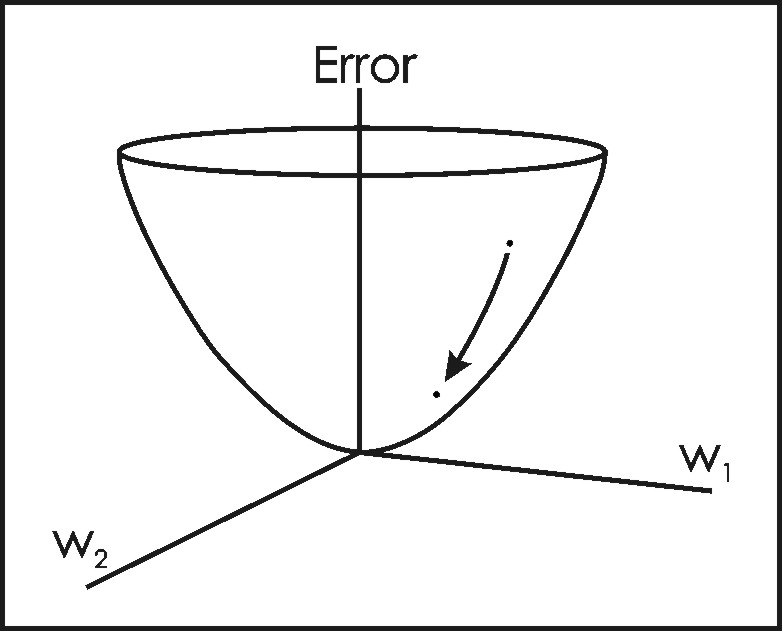
\includegraphics[scale=0.3]{CNN_loss}
\end{center}

A $dL/dW$ matematikai egyenlet írjuk fel a veszteség hozzájárulást. Következő lépés a hiba visszaterjesztés, amely meghatározza, hogy a súlyok milyen mértékben járultak hozzá a veszteséghez, és megtalálják azokat a módokat, amelyekkel a károk csökkenthetők. Miután kiszámítjuk ezt a származékot, akkor megyünk az utolsó lépéshez, amely a súlyok frissítése. Itt vesszük az összes súlyt és szűröt, és frissítjük őket úgy, hogy a gradiens ellenkező irányba változzon.

\begin{center}
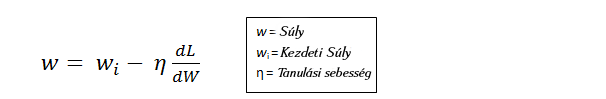
\includegraphics[scale=0.9]{CNN_update_weight}
\end{center}

A tanulási sebesség egy olyan paraméter, amelyet a programozó választ. A magas tanulási arány azt jelenti, hogy nagyobb súlycsökkenést kell végrehajtani a súlycsökkentésekben, így kevesebb időre lehet szükség ahhoz, hogy a modell konvergáljon az optimális súlycsoporton. Azonban a túl magas tanulási arány olyan túl nagy ugrásokhoz vezethet, amelyek nem elég pontosak ahhoz, hogy elérjék az optimális pontot.

\begin{center}
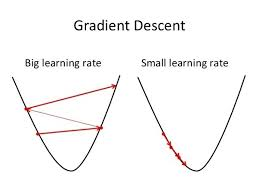
\includegraphics[scale=0.7]{CNN_learning_rate}
\end{center}

Az előre terjesztés, a veszteség számítás, a visszaterjesztés és a paraméterfrissítés folyamata egy képzési iteráció. A program megismételi ezt a folyamatot egy rögzített számú iterációra. Miután befejezte a paraméter frissítést az utolsó képzésnél, remélhetőleg a hálózat megfelelően működik.\\

\begin{flushleft}
\textit{\textbf{Tesztelés}}
\end{flushleft}

Végül megnézzük, hogy működik-e a hálózat vagy sem. Különböző (még nem látott) képeket továbbíthatunk a CNN-en keresztül. Összehasonlítjuk a kimeneteket a címkékkel, és megnézzük a hibát. Ha alacsony hibát kapunk a hálózat jól dolgozott.

\begin{flushleft}
{\Large Transfer learning}
\end{flushleft}

A konvolúciós hálózatok betanításához nagyszámú mintára és nagyteljesítményű számítógépekre van szükség. Amennyiben nem áll rendelkezésünkre nagyjából egymillió képkockából álló tanító adathalmaz, akkor kisszámú mintáról beszélünk. Ha nincs lehetőségünk vagy erőforrásunk nagy adathalmazzal tanítani, akkor is megvalósíthatjuk a kívánt leképezést. A transfer learning (tanulás átadása) módszer segítségével egy előre betanított hálózatot veszünk alapul, és annak utolsó pár rétegét lecserélve végezzük a tanítást. Ilyenkor a megmaradt rétegek betanított tulajdonság érzékelő funkciója segítségével a lecserélt rétegek által megvalósítandó leképezés könnyebbé vállhat. A konvolúciós neurális hálózatok tanítása esetében ez egy gyakori eljárás. A weben számos előre betanított hálózat található.\\

!KIEGÉSZÍTÉS!
\textit{Tanító mintapontok előállítása
A megvalósító neurális hálózat betanítása felügyelt tanulás módszerrel történik. A minták alapján történő tanulás lényege, hogy az eljárás során a be és kimeneti mintapárokból igyekszünk megfelelő ismereteket kinyerni és ezzel a rendszer viselkedését módosítani. A hálózat feladata, hogy megtanulja a rendelkezésre álló mintapont párok által reprezentált bemenet-kimenet leképezést. Ehhez elő kell állítani a megfelelő adathalmazt.}